% Complete DistilGPT-2 evaluation path combined with detailed block.
\usetikzlibrary{arrows.meta,calc,positioning}
\definecolor{gptpanel}{RGB}{237,243,248}
\definecolor{gptattention}{RGB}{252,229,207}
\definecolor{gptmlp}{RGB}{226,239,204}
\definecolor{gptreduction}{RGB}{255,244,204}
\definecolor{gptresidual}{RGB}{76,101,125}

\begin{figure}[t]
  \centering
  \resizebox{0.99\linewidth}{!}{%
    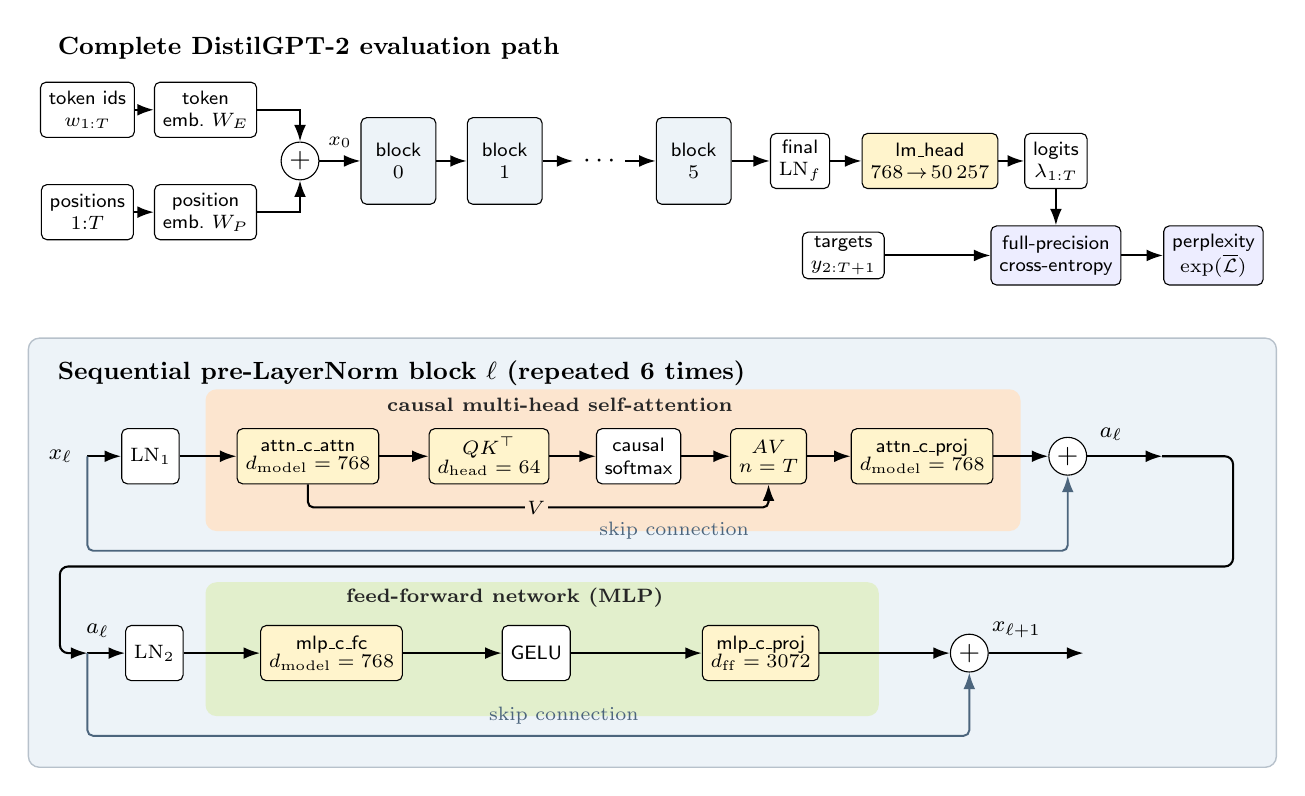
\begin{tikzpicture}[
      x=1cm,
      y=1cm,
      font=\sffamily\footnotesize,
      >={Latex[length=2.1mm,width=1.5mm]},
      flow/.style={->,line width=0.75pt},
      residual/.style={->,line width=0.7pt,draw=gptresidual},
      tie/.style={<->,densely dashed,line width=0.65pt,draw=gptresidual},
      operation/.style={
          draw,
          rounded corners=2pt,
          fill=white,
          minimum height=7mm,
          inner xsep=3pt,
          inner ysep=1.5pt,
          align=center,
          font=\sffamily\scriptsize
        },
      reduction/.style={operation,fill=gptreduction},
      block/.style={operation,fill=gptpanel,minimum width=9.5mm,minimum height=11mm},
      metric/.style={operation,fill=blue!7,minimum height=7.5mm},
      add/.style={
          circle,
          draw,
          fill=white,
          minimum size=4.8mm,
          inner sep=0pt,
          font=\normalsize
        }
      ]

% ==================================================================
      % TOP PANEL: Complete DistilGPT-2 evaluation path (no background)
      % ==================================================================
      \node[anchor=north west,font=\bfseries\small]
      at (0.05, 8.05) {Complete DistilGPT-2 evaluation path};

      % Input embeddings
      \node[operation] (tokens) at (0.55, 7.00) {token ids\\$w_{1:T}$};
      \node[operation] (positions) at (0.55, 5.70) {positions\\$1{:}T$};
      \node[operation] (wte) at (2.05, 7.00) {token\\emb.\ $W_E$};
      \node[operation] (wpe) at (2.05, 5.70) {position\\emb.\ $W_P$};
      \node[add] (embadd) at (3.25, 6.35) {$+$};

      % Transformer blocks stack (highlighted with gptpanel blue fill)
      \node[block] (bzero) at (4.50, 6.35) {block\\$0$};
      \node[block] (bone) at (5.85, 6.35) {block\\$1$};
      \node[draw=none,font=\bfseries] (dots) at (7.05, 6.35) {$\cdots$};
      \node[block] (bfive) at (8.25, 6.35) {block\\$5$};

      % Head & Logits
      \node[operation] (lnf) at (9.60, 6.35) {final\\$\mathrm{LN}_f$};
      \node[reduction] (head) at (11.25, 6.35) {\code{lm\_head}\\$768\!\to\!50\,257$};
      \node[operation] (logits) at (12.85, 6.35) {logits\\$\lambda_{1:T}$};

      % Evaluation metrics
      \node[operation,minimum height=5.5mm] (targets) at (10.15, 5.15) {targets\\$y_{2:T+1}$};
      \node[metric] (loss) at (12.85, 5.15) {full-precision\\cross-entropy};
      \node[metric] (ppl) at (14.85, 5.15) {perplexity\\$\exp(\overline{\mathcal L})$};

      % Connections in top panel
      \draw[flow] (tokens) -- (wte);
      \draw[flow] (positions) -- (wpe);
      \draw[flow] (wte.east) -| (embadd.north);
      \draw[flow] (wpe.east) -| (embadd.south);

      \draw[flow] (embadd) -- node[above=1pt,font=\scriptsize] {$x_0$} (bzero);
      \draw[flow] (bzero) -- (bone);
      \draw[flow] (bone) -- (dots);
      \draw[flow] (dots) -- (bfive);
      \draw[flow] (bfive) -- (lnf);
      \draw[flow] (lnf) -- (head);
      \draw[flow] (head) -- (logits);

      % Metrics connections
      \draw[flow] (logits) -- (loss);
      \draw[flow] (targets) -- (loss);
      \draw[flow] (loss) -- (ppl);


      % ==================================================================
      % BOTTOM PANEL: One sequential pre-LayerNorm block (zoomed, gptpanel blue)
      % ==================================================================
      \fill[gptpanel,rounded corners=4pt,draw=gptresidual!40,line width=0.5pt]
      (-0.20, -1.35) rectangle (15.65, 4.10);

      \node[anchor=north west,font=\bfseries\small]
      at (0.05, 3.93) {Sequential pre-LayerNorm block $\ell$ (repeated 6 times)};

      % --- Attention sublayer ---
      \fill[gptattention,rounded corners=4pt]
      (2.05, 1.65) rectangle (12.40, 3.45);
      \node[font=\bfseries\scriptsize,text=black!85]
      at (6.55, 3.25) {causal multi-head self-attention};

      \coordinate (xin) at (0.55, 2.60);
      \node[anchor=east] at (0.48, 2.60) {$x_\ell$};
      \node[operation] (lnone) at (1.35, 2.60) {$\mathrm{LN}_1$};
      \node[reduction] (cattn) at (3.35, 2.60)
      {\code{attn\_c\_attn}\\[-0.45mm]$d_{\rm model}=768$};
      \node[reduction] (qk) at (5.65, 2.60)
      {$QK^\top$\\[-0.45mm]$d_{\rm head}=64$};
      \node[operation] (softmax) at (7.55, 2.60)
      {causal\\softmax};
      \node[reduction] (av) at (9.20, 2.60)
      {$AV$\\[-0.45mm]$n=T$};
      \node[reduction] (attnproj) at (11.15, 2.60)
      {\code{attn\_c\_proj}\\[-0.45mm]$d_{\rm model}=768$};
      \node[add] (addone) at (13.00, 2.60) {$+$};
      \coordinate (amid) at (14.20, 2.60);
      \node[anchor=south] at (13.55, 2.67) {$a_\ell$};

      \draw[flow] (xin) -- (lnone.west);
      \draw[flow] (lnone.east) -- (cattn.west);
      \draw[flow] (cattn.east) -- (qk.west);
      \draw[flow] (qk.east) -- (softmax.west);
      \draw[flow] (softmax.east) -- (av.west);
      \draw[flow,rounded corners=2pt]
      (cattn.south) -- (3.35, 1.95) -- (9.20, 1.95) -- (av.south);
      \node[font=\scriptsize,fill=gptattention,inner sep=1pt]
      at (6.25, 1.95) {$V$};
      \draw[flow] (av.east) -- (attnproj.west);
      \draw[flow] (attnproj.east) -- (addone.west);
      \draw[flow] (addone.east) -- (amid);

      % Attention skip connection (below the orange box)
      \draw[residual,rounded corners=2pt]
      (xin) -- (0.55, 1.40) -- (13.00, 1.40) -- (addone.south);
      \node[anchor=south,draw=none,font=\scriptsize,text=gptresidual]
      at (8.00, 1.42) {skip connection};

      % --- MLP sublayer ---
      \fill[gptmlp,rounded corners=4pt]
      (2.05, -0.70) rectangle (10.60, 1.00);
      \node[font=\bfseries\scriptsize,text=black!85]
      at (5.85, 0.80) {feed-forward network (MLP)};

      \coordinate (ain) at (0.55, 0.10);
      \node[anchor=south] at (0.68, 0.18) {$a_\ell$};
      \node[operation] (lntwo) at (1.40, 0.10) {$\mathrm{LN}_2$};
      \node[reduction] (fc) at (3.65, 0.10)
      {\code{mlp\_c\_fc}\\[-0.45mm]$d_{\rm model}=768$};
      \node[operation,fill=white] (gelu) at (6.25, 0.10) {GELU};
      \node[reduction] (mlpproj) at (9.10, 0.10)
      {\code{mlp\_c\_proj}\\[-0.45mm]$d_{\rm ff}=3072$};
      \node[add] (addtwo) at (11.75, 0.10) {$+$};
      \coordinate (xout) at (13.20, 0.10);
      \node[anchor=south] at (12.35, 0.17) {$x_{\ell+1}$};

      \draw[flow] (ain) -- (lntwo.west);
      \draw[flow] (lntwo.east) -- (fc.west);
      \draw[flow] (fc.east) -- (gelu.west);
      \draw[flow] (gelu.east) -- (mlpproj.west);
      \draw[flow] (mlpproj.east) -- (addtwo.west);
      \draw[flow] (addtwo.east) -- (xout);

      % MLP skip connection
      \draw[residual,rounded corners=2pt]
      (ain) -- (0.55, -0.95) -- (11.75, -0.95) -- (addtwo.south);
      \node[anchor=south,draw=none,font=\scriptsize,text=gptresidual]
      at (6.60, -0.93) {skip connection};

      % Sublayer-to-sublayer transition arrow (amid -> ain)
      \draw[flow,rounded corners=3pt]
      (amid) -- (15.10, 2.60) -- (15.10, 1.20) --
      (0.20, 1.20) -- (0.20, 0.10) -- (ain);

        \end{tikzpicture}%
  }
  \caption{Complete DistilGPT-2 architecture and evaluation path. Token and
    position embeddings form $x_0$, which passes sequentially through six
    pre-LayerNorm GPT-2 blocks. The lower panel expands the
    repeated block into its attention and MLP sublayers. Yellow nodes identify the groups
    instrumented by the rounding experiments.}
  \label{fig:architecture}
\end{figure}
